\documentclass[12pt]{exam}
\usepackage{amsmath}
\printanswers

\usepackage{pgf,tikz,pgfplots}
\pgfplotsset{compat=1.15}
\usepackage{mathrsfs}
\usetikzlibrary{arrows}

\begin{document}

\begin{questions}

% Question 1
\question Clasifica los siguientes números indicando a cuáles de los conjuntos \( \mathbb{N}, \mathbb{Z}, \mathbb{Q} \) o \( \mathbb{R} \) pertenecen:
\[
-\frac{58}{45}, \frac{51}{17}, \pi, \frac{\sqrt{3}}{4}, \frac{3}{8}, \sqrt{5}, \frac{2}{3}, 1.07
\]

% Question 2
\question Expresa en forma de intervalo y haz la representación en cada caso.
\begin{parts}
    \part \( |x| \geq 8 \)
    \part \( |x - 4| < 5 \)
\end{parts}

% Question 3
\question Dos esferas metálicas de \( 1000 \, \text{kg} \) cada una se atraen con una fuerza de \( 8.35 \cdot 10^{-9} \, \text{N} \). ¿A qué distancia se encuentran sus centros? Aplica la Ley de Gravitación Universal:
\[
F = G \frac{M m}{r^2} \quad \text{donde} \quad G = 6.67 \cdot 10^{-11} \, \frac{\text{N} \cdot \text{m}^2}{\text{kg}^2}
\]
Acota el error cometido.

% Question 4
\question Aplica la definición de logaritmo y obtén \( x \).
\begin{parts}
    \part \( \log_3 x = -\frac{1}{4} \)
    \part \( \ln \frac{x}{3} = -1 \)
    \part \( \log_{x} 512 = 3 \)
\end{parts}

% Question 5
\question Aplica las propiedades de los logaritmos y halla \( A \).
\[
\log A = 2 \log 3 + 0.5 \log 4 - 3 \log 2
\]

% Question 6
\question Calcula \( x \) en cada caso.
\begin{parts}
    \part \( 2.5^x = 0.0087 \)
    \part \( e^x = 425 \)
\end{parts}

% Question 7
\question Determina los términos \( a_1, a_{97} \) y \( a_{500} \) de la sucesión cuyo término general es:
\[
a_n = \frac{n^2 - 709}{n + 3}
\]

% Question 8
\question Escribe los diez primeros términos de la sucesión definida así: \( a_1 = 4 \), \( a_2 = 7 \), \( a_{n+2} = 2a_{n} - a_{n+1} \).

% Question 9
\question Halla el término general de las siguientes sucesiones. Indica cuáles de ellas son progresiones aritméticas y cuáles progresiones geométricas:
\begin{parts}
    \part \( 3, 7, 11, 15, 19, 23, \ldots \)
    \part \( 1, 2, 5, 10, 17, 26, \ldots \)
    \part \( 1, 024, 512, 256, 128, \ldots \)
    \part \( 3, -9, 27, -81, 243, \ldots \)
    \part \( 8/13, 19/52, 3/26, -7/52, \ldots \)
\end{parts}

% Question 10
\question Halla la ley de recurrencia que define estas sucesiones:
\begin{parts}
    \part \( 7, 8, 15, 23, 38, 61, 99, \ldots \)
    \part \( 1, 1, 1, 3, 5, 9, 17, 31, \ldots \)
    \part \( 0, 1, 2, 3, 6, 11, 20, 37, \ldots \)
    \part \( 0, 1, 3, 6, 10, 15, 21, \ldots \)
\end{parts}

% Question 11
\question En una progresión aritmética, \( a_{15} = 43 \) y \( a_{86} = 85.6 \).
\begin{parts}
    \part Calcula \( S_{100} \).
    \part Obtén el valor de \( a_{220} \).
\end{parts}

% Question 12
\question Dados estos dos términos de una sucesión, \( a_1 = 2 \) y \( a_3 = 8 \), halla cuatro términos más y el término general suponiendo que se trata de una progresión:
\begin{parts}
    \part aritmética
    \part geométrica
\end{parts}


% Question 1
\question Resuelve factorizando previamente.
\[
3x^5 + x^4 - 9x^3 - 9x^2 - 2x = 0
\]

% Question 2
\question Opera y simplifica el resultado.
\begin{parts}
    \part \( \frac{x^2}{x^2 - 1} - \frac{x}{x + 1} \)
    \part \( \frac{3x}{x - 1} \)
\end{parts}

% Question 3
\question Resuelve las siguientes ecuaciones:
\begin{parts}
    \part \( x^4 - 3x^2 + 2 = 0 \)
    \part \( \sqrt{8 + 2x} - x = x + 6 \)
    \part \( \frac{3x}{x^2 - 4} = \frac{x}{x + 2} - \frac{4}{3} \)
    \part \( 3^x - 1 = \frac{1}{\sqrt{3}} \)
    \part \( 2^{2x} - 6 \cdot 2^x + 8 = 0 \)
    \part \( \ln x + \ln 4 = 2 \ln (x + 1) \)
    \part \( |3x + 1| = |x - 3| \)
\end{parts}

% Question 4
\question Resuelve estos sistemas no lineales:
\begin{parts}
    \part \( \begin{cases} xy - x^2 = 6 \\ x + y = 7 \end{cases} \)
    \part \( \begin{cases} x^2 + y^2 + xy = 1 \\ 2x^2 - y^2 - xy = 2 \end{cases} \)
\end{parts}

% Question 5
\question Resuelve estos sistemas de ecuaciones:
\begin{parts}
    \part \( \begin{cases} y - 2x = 0 \\ 3y - 6 \cdot 3^x = -9 \end{cases} \)
    \part \( \begin{cases} x^2 + 5 = y + 2 \\ \log 5x - \log y = 1 \end{cases} \)
    \part \( \begin{cases} x + y = 2 \\ x - y = 1 \\ 2y + 3z = -1 \end{cases} \)
    \part \( \begin{cases} x + 2y + 2z = 3 \\ x + y + 3z = 5 \\ -2x + 3y + 3z = 1 \end{cases} \)
\end{parts}

% Question 6
\question Resuelve estos sistemas de inecuaciones:
\begin{parts}
    \part \( \begin{cases} 2x + y \leq 5 \\ -x - y \leq 5 \\ y \leq 4 \\ x \geq -2 \end{cases} \)
    \part \( \begin{cases} x^2 - x - 6 \leq 0 \\ \frac{x^2 - 5x + 3}{2} < -3 \end{cases} \)
\end{parts}

% Question 7
\question Resuelve.
\begin{parts}
    \part \( x (x - 1) - 2 (x + 2) < x (x + 1) \)
    \part \( \frac{x^2 + 2x + 1}{x + 3} \geq 0 \)
\end{parts}

% Question 8
\question Un circo está compuesto por tres pistas circulares tangentes dos a dos. Las distancias entre sus centros son 80, 100 y 120 metros, respectivamente. Calcula el diámetro de cada una de las pistas.


% Question 1
\question Clasifica los siguientes números indicando a cuáles de los conjuntos \( \mathbb{N}, \mathbb{Z}, \mathbb{Q} \) o \( \mathbb{R} \) pertenecen:
\[
-\frac{27}{18}, \frac{35}{7}, e, \frac{\sqrt{7}}{5}, \frac{9}{16}, \sqrt{10}, \frac{5}{8}, 2.56
\]
\begin{solution}
\text{Números: } \mathbb{Q}, \mathbb{R}, \text{ etc.}
\end{solution}

% Question 2
\question Expresa en forma de intervalo y haz la representación en cada caso.
\begin{parts}
    \part \( |x| < 6 \)
    \part \( |x + 2| \geq 3 \)
\end{parts}
\begin{solution}
\text{Intervalos: } (-6, 6), (-5, 1) \text{ y } (-1, 5)
\end{solution}

% Question 3
\question Dos cuerpos metálicos de \( 800 \, \text{kg} \) cada uno se atraen con una fuerza de \( 7.85 \cdot 10^{-9} \, \text{N} \). ¿A qué distancia se encuentran sus centros?
\[
F = G \frac{M m}{r^2} \quad \text{donde} \quad G = 6.67 \cdot 10^{-11} \, \frac{\text{N} \cdot \text{m}^2}{\text{kg}^2}
\]
\begin{solution}
r \approx 14.65 \text{ m}
\end{solution}

% Question 4
\question Aplica la definición de logaritmo y obtén \( x \).
\begin{parts}
    \part \( \log_2 x = -\frac{1}{3} \)
    \part \( \ln \frac{x}{5} = -2 \)
    \part \( \log_{x} 256 = 4 \)
\end{parts}
\begin{solution}
x \approx 0.7937, \, 0.75, \, 4
\end{solution}

% Question 5
\question Aplica las propiedades de los logaritmos y halla \( A \).
\[
\log A = 3 \log 2 + 0.7 \log 5 - 4 \log 3
\]
\begin{solution}
A \approx 0.083
\end{solution}

% Question 6
\question Calcula \( x \) en cada caso.
\begin{parts}
    \part \( 3^x = 0.027 \)
    \part \( e^x = 210 \)
\end{parts}
\begin{solution}
x \approx -3, \, 5.3
\end{solution}

% Question 7
\question Determina los términos \( a_1, a_{50} \) y \( a_{200} \) de la sucesión cuyo término general es:
\[
a_n = \frac{2n^2 - 405}{n - 2}
\]
\begin{solution}
a_1 = -203, \, a_{50} = 103, \, a_{200} = 128
\end{solution}

% Question 8
\question Escribe los diez primeros términos de la sucesión definida así: \( a_1 = 3 \), \( a_2 = 10 \), \( a_{n+2} = 3a_{n} - a_{n+1} \).
\begin{solution}
3, 10, 27, 66, 159, 390, 939, \ldots
\end{solution}

% Question 9
\question Halla el término general de las siguientes sucesiones. Indica cuáles de ellas son progresiones aritméticas y cuáles progresiones geométricas:
\begin{parts}
    \part \( 4, 9, 14, 19, 24, 29, \ldots \)
    \part \( 2, 3, 6, 11, 18, 27, \ldots \)
    \part \( 2, 64, 16, 4, 1, \ldots \)
    \part \( 2, -6, 18, -54, 162, \ldots \)
    \part \( 10/19, 21/38, 4/19, -5/38, \ldots \)
\end{parts}
\begin{solution}
\text{PA: 1. } a_n = 5n - 1; \, \text{SG: 3. } a_n = 2^n; \text{ otros no son PA ni SG.}
\end{solution}

% Question 10
\question Halla la ley de recurrencia que define estas sucesiones:
\begin{parts}
    \part \( 5, 6, 11, 17, 28, 45, 73, \ldots \)
    \part \( 2, 2, 2, 4, 8, 14, 26, 48, \ldots \)
    \part \( 0, 2, 4, 6, 10, 16, 26, \ldots \)
    \part \( 1, 2, 4, 7, 11, 16, 22, \ldots \)
\end{parts}
\begin{solution}
\text{1. } a_{n+2} = a_{n+1} + a_n; \, \text{2. } a_{n+2} = 2a_{n+1} - a_n.
\end{solution}

% Question 11
\question En una progresión aritmética, \( a_{10} = 35 \) y \( a_{75} = 100 \).
\begin{parts}
    \part Calcula \( S_{50} \).
    \part Obtén el valor de \( a_{150} \).
\end{parts}
\begin{solution}
S_{50} = 2625, \, a_{150} = 165
\end{solution}

% Question 12
\question Dados estos dos términos de una sucesión, \( a_1 = 3 \) y \( a_4 = 27 \), halla cuatro términos más y el término general suponiendo que se trata de una progresión:
\begin{parts}
    \part aritmética
    \part geométrica
\end{parts}
\begin{solution}
\text{Aritmética: } a_n = 3 + (n-1) \cdot 8; \, \text{Geométrica: } a_n = 3 \cdot 3^{n-1}
\end{solution}

% Question 1
\question Resuelve factorizando previamente.
\[
4x^4 - 8x^3 + 2x^2 - 6x = 0
\]
\begin{solution}
x = 0, \, 1, \, 2
\end{solution}

% Question 2
\question Opera y simplifica el resultado.
\begin{parts}
    \part \( \frac{x^2 + 2}{x^2 + 3} - \frac{x + 1}{x + 2} \)
    \part \( \frac{5x}{x + 2} \)
\end{parts}
\begin{solution}
\text{Simplificación: } \text{Resultado 1: } \frac{-x}{x^2 + 3}; \, \text{Resultado 2: } 5
\end{solution}

% Question 3
\question Resuelve las siguientes ecuaciones:
\begin{parts}
    \part \( x^3 - 5x + 6 = 0 \)
    \part \( \sqrt{7 + 3x} - x = x + 1 \)
    \part \( \frac{2x}{x^2 - 9} = \frac{x}{x - 3} - \frac{3}{2} \)
    \part \( 4^x - 2 = \frac{1}{2} \)
    \part \( 3^{2x} - 9 \cdot 3^x + 18 = 0 \)
    \part \( \ln(2x) + \ln(3) = 3 \ln(x) \)
    \part \( |2x - 4| = |x + 1| \)
\end{parts}
\begin{solution}
\text{Respuestas: } x = -3, 2, 5; \, x = 3; \, x = 0; \, x = -1; \, x = 2.
\end{solution}

% Question 4
\question Resuelve estos sistemas no lineales:
\begin{parts}
    \part \( \begin{cases} xy - x^2 = 7 \\ x + y = 8 \end{cases} \)
    \part \( \begin{cases} x^2 + y^2 + xy = 2 \\ 3x^2 - y^2 - xy = 3 \end{cases} \)
\end{parts}
\begin{solution}
\text{Sistema 1: } (x, y) = (7, 1), (5, 3); \, \text{Sistema 2: } (x, y) = (1, 1), (0, 1).
\end{solution}

% Question 5
\question Resuelve estos sistemas de ecuaciones:
\begin{parts}
    \part \( \begin{cases} y - 3x = 1 \\ 2y - 3 \cdot 2^x = -6 \end{cases} \)
    \part \( \begin{cases} x^2 - 4 = y - 1 \\ \log(3x) - \log(y) = 0 \end{cases} \)
    \part \( \begin{cases} x + y = 5 \\ x - y = 2 \\ 3y + 4z = 2 \end{cases} \)
    \part \( \begin{cases} 2x + 3y + z = 7 \\ 3x + y + 2z = 8 \\ -x + 4y + z = 5 \end{cases} \)
\end{parts}
\begin{solution}
\text{Respuestas: } (x, y) = (2, 3); \, (x, y) = (3, 2); \, (x, y, z) = (3, 2, -1); \, (x, y, z) = (1, 1, 2).
\end{solution}

% Question 6
\question Resuelve estos sistemas de inecuaciones:
\begin{parts}
    \part \( \begin{cases} 3x + 2y \leq 12 \\ -2x - y \leq 6 \\ y \leq 7 \\ x \geq 0 \end{cases} \)
    \part \( \begin{cases} x^2 - 5x + 6 \leq 0 \\ \frac{x^2 - 4x + 1}{2} < 0 \end{cases} \)
\end{parts}
\begin{solution}
\text{Sistema 1: } (x, y) \text{ en ciertos valores.} \, \text{Sistema 2: } x \in (1, 4).
\end{solution}

% Question 7
\question Resuelve.
\begin{parts}
    \part \( x (x + 3) - 5 (x - 1) < x (x + 2) \)
    \part \( \frac{x^2 - 5x + 6}{x - 2} \geq 0 \)
\end{parts}
\begin{solution}
x < -1, \, x \geq 3
\end{solution}

% Question 8
\question Un parque tiene tres áreas circulares tangentes dos a dos. Las distancias entre sus centros son 90, 110 y 130 metros, respectivamente. Calcula el diámetro de cada una de las áreas.
\begin{solution}
\text{Diámetros: } 30, 40, 50 \text{ m.}
\end{solution}


% Segunda tanda

\textbf{Triángulos, trigonometría y complejos}

\question Expresa, a través de las razones trigonométricas de un ángulo del primer cuadrante, las razones trigonométricas de los siguientes ángulos:  
\( 154^\circ, \; 207^\circ, \; 318^\circ, \; 2456^\circ \).

\question Si \( \sin \alpha = \frac{4}{5} \) y \( \alpha > 90^\circ \), calcula sin hallar el ángulo \( \alpha \):  
\begin{parts}
    \part \( \cos \alpha \)
    \part \( \tan \alpha \)
    \part \( \sin (180^\circ + \alpha) \)
    \part \( \cos (90^\circ + \alpha) \)
    \part \( \tan (180^\circ - \alpha) \)
    \part \( \sin (90^\circ - \alpha) \)
\end{parts}

\question Si \( \tan \alpha = -3.5 \), halla \( \alpha \) con ayuda de la calculadora, exprésalo como un ángulo del intervalo \( [0^\circ, 180^\circ) \) y obtén su seno y su coseno.

\question Las bases de un trapecio isósceles miden \( 18 \, \text{cm} \) y \( 26 \, \text{cm} \), y los lados iguales \( 14 \, \text{cm} \). Calcula sus ángulos y su área.

\question Resuelve el triángulo \( \triangle ABC \) y halla su área en estos casos:  
\begin{parts}
    \part \( c = 19 \, \text{cm}, \; a = 33 \, \text{cm}, \; \hat{B} = 48^\circ \)
    \part \( a = 15 \, \text{cm}, \; b = 11 \, \text{cm}, \; \hat{B} = 30^\circ \)
\end{parts}

\question El radar de un barco detecta un objeto no identificado a \( 40 \, \text{m} \) de profundidad y en una dirección que forma \( 15^\circ \) con la horizontal. ¿Qué distancia tiene que recorrer un buzo para llegar desde el barco hasta el objeto?

\question Desde la terraza de un edificio de \( 150 \, \text{m} \) de altura medimos los ángulos que se indican en la figura. Calcula: 

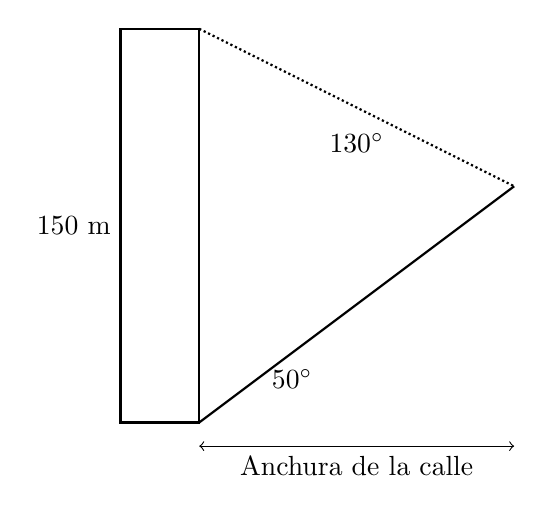
\begin{tikzpicture}
    % Edificio
    \draw[thick] (0,0) -- (0,5) -- (1,5) -- (1,0) -- cycle;
    \draw[thick, densely dotted] (1,5) -- (5,3); % Línea hacia la hipotenusa
    \draw[thick] (5,3) -- (1,0); % Línea hacia el punto inferior

    % Medidas y ángulos
    \node[left] at (0,2.5) {150 m}; % Altura del edificio
    \node[below] at (3,3.8) {$130^\circ$}; % Ángulo superior
    \node[below right] at (1.8,0.8) {$50^\circ$}; % Ángulo inferior

    % Anotación de base
    \draw[<->] (1,-0.3) -- (5,-0.3);
    \node[below] at (3,-0.3) {Anchura de la calle};
\end{tikzpicture}
\begin{parts}
    \part La altura del edificio más bajo.
    \part La anchura de la calle.
\end{parts}

\question Los lados de un paralelogramo miden \( 18 \, \text{cm} \) y \( 32 \, \text{cm} \) y forman un ángulo de \( 52^\circ \). Halla la longitud de la diagonal mayor.

\question De esta figura, sabemos que  
\[
BD = DC, \; \hat{A} = 60^\circ, \; \hat{ADB} = 45^\circ, \; AD = 5 \, \text{m}.
\]  
Calcula \( BC \).

\end{questions}



\end{document}
